\documentclass[10pt,twocolumn]{article}
\usepackage[a4paper,margin=0.55in,columnsep=0.22in]{geometry}
\usepackage[T1]{fontenc}
\usepackage{lmodern}
\usepackage{amsmath,amssymb}
\usepackage{graphicx}
\usepackage{booktabs}
\usepackage{xcolor}
\usepackage{tikz}
\usetikzlibrary{positioning,arrows.meta,fit}
\usepackage[hidelinks]{hyperref}
\usepackage[font=small,labelfont=bf,skip=3pt]{caption}
\usepackage{enumitem}
\setlist{nosep,leftmargin=*}
\setlength{\parskip}{1pt}
\setlength{\textfloatsep}{6pt}
\setlength{\floatsep}{5pt}
\setlength{\dbltextfloatsep}{6pt}
\setlength{\abovedisplayskip}{3pt}
\setlength{\belowdisplayskip}{3pt}
\graphicspath{{figures/}}
\definecolor{ppo}{HTML}{2A78D6}
\definecolor{mpc}{HTML}{EB6834}
\definecolor{priv}{HTML}{8A8984}
\makeatletter
\renewcommand\section{\@startsection{section}{1}{\z@}{-1.0ex plus -.5ex}{0.4ex}{\normalfont\normalsize\bfseries}}
\renewcommand\subsection{\@startsection{subsection}{2}{\z@}{-0.6ex}{0.2ex}{\normalfont\small\bfseries}}
\makeatother

\title{\vspace{-1.6em}\Large\textbf{Adaptive Bitrate Streaming with PPO and an Asymmetric Critic}\vspace{-0.6em}}
\author{Neeraj Kumar (B23CS1044) \quad\textbar\quad Abhyudaya Tiwari (B23CS1085)\\[2pt]
  GitHub: \url{https://github.com/nk1044/ai-assignment2}\vspace{-1.2em}}
\date{}

\begin{document}
\maketitle

\section{Problem}
Video players (DASH/HLS) download a video as 4-second \emph{chunks}, each available at several bitrates.
Before every chunk, an \emph{adaptive bitrate} (ABR) controller must pick a quality while the network
bandwidth fluctuates unpredictably. The three goals conflict:
\begin{itemize}
  \item too high a bitrate drains the playback buffer and the video \textbf{stalls};
  \item too low a bitrate wastes bandwidth on a blurry picture;
  \item frequent changes cause visible flicker.
\end{itemize}
Decisions have delayed consequences: buffer saved now prevents a stall tens of seconds later. ABR is
therefore a sequential decision problem under uncertainty, which we solve with reinforcement learning.
Classic heuristics (rate-, buffer- and model-predictive control) appear only as baselines.

\begin{table*}[t]
\centering\footnotesize
\caption{Mean QoE per chunk on unseen test traces (higher is better): HSDPA 3G (142 traces), FCC broadband
(12) and stress tests (30; 5 generated scenarios $\times$ 6 variants, of which 6 are metro tunnels).
$\Delta$ is relative to RobustMPC on HSDPA. Stall time (s) and quality switches are per video on HSDPA.}
\label{tab:results}
\setlength{\tabcolsep}{5pt}
\begin{tabular}{lccccccc}
\toprule
Method & HSDPA & $\Delta$ vs.\ RobustMPC & Stall [s] & Switches & FCC & Stress tests & Metro tunnel\\
\midrule
\textit{Offline optimal (knows the future)} & \textit{1.145} & \textit{+26\,\%} & 0.01 & 2.4 & \textit{0.819} & \textit{1.716} & \textit{2.11}\\
\midrule
\textbf{PPO, asymmetric critic (final)} & \textbf{0.971} & \textbf{+7\,\%} & 0.35 & \textbf{4.5} & \textbf{0.675} & \textbf{1.393} & \textbf{1.37}\\
A2C v1, symmetric critic & 0.934 & +3\,\% & 0.17 & 12.1 & 0.644 & 1.047 & 0.16\\
A2C v2, symmetric critic & 0.924 & +2\,\% & 0.35 & 11.5 & 0.645 & 0.926 & $-$0.50\\
\midrule
RobustMPC & 0.907 & -- & 0.91 & 9.5 & 0.604 & 0.738 & $-$1.79\\
BOLA & 0.770 & $-$15\,\% & 0.01 & 13.8 & 0.396 & 1.113 & 1.27\\
RB (rate-based) & 0.745 & $-$18\,\% & 1.13 & 6.5 & 0.428 & 1.042 & 0.37\\
BB (buffer-based) & 0.626 & $-$31\,\% & 1.80 & 25.3 & 0.344 & 0.602 & $-$1.12\\
FastMPC & 0.431 & $-$52\,\% & 6.82 & 10.6 & 0.252 & 0.330 & $-$3.24\\
\bottomrule
\end{tabular}
\end{table*}

\section{RL Formulation}
\textbf{Step} $=$ one chunk decision; \textbf{episode} $=$ one video of $N{=}48$ chunks (3.2\,min)
streamed over one bandwidth trace; $\gamma=0.99$.

\textbf{State} $s_t\in\mathbb{R}^{6\times 8}$ (25 informative values):
\begin{itemize}
  \item the last bitrate ($\div4300$\,kbps) and the buffer level ($\div10$\,s);
  \item the throughput (Mbps) and download time ($\div10$\,s) of the last 8 chunks;
  \item the size of the next chunk at each of the 6 bitrates (MB);
  \item the fraction of chunks remaining.
\end{itemize}
Future bandwidth is hidden, so the agent faces a POMDP. The 8-step histories are the standard
approximate-Markov summary. The remaining-chunk count lets the agent spend surplus buffer near the end.

\textbf{Action} $a_t\in\{0,\dots,5\}$ (discrete): \{300, 750, 1200, 1850, 2850, 4300\}\,kbps, the ladder
of the EnvivioDash3 reference video.

\textbf{Reward} (QoE$_{\text{lin}}$, as used by MPC and Pensieve):
\begin{equation}
r_t = q(R_t) - \mu\,T_t - \lvert q(R_t)-q(R_{t-1})\rvert ,
\end{equation}
where $q(R)=R$ in Mbps, $\mu=4.3$ and $T_t$ is the stall time (s) caused by chunk $t$. Setting $\mu$ equal to the top bitrate makes 1\,s of
stall cost as much as a top-quality chunk earns, so stalling is never worth it. The smoothness term
penalises jumps in proportion to their size. Summed over an episode, the reward equals the evaluation
metric exactly.

\textbf{Environment.} A chunk-level, trace-driven simulator replays \emph{real} recorded bandwidth:
\begin{itemize}
  \item 68/142 Norway HSDPA 3G commute traces (train/test) and 47/12 FCC broadband traces;
  \item the real per-chunk sizes of the reference video.
\end{itemize}
Each transition works as follows:
\begin{itemize}
  \item download time $d_t$ = the chunk's bytes integrated over the trace (95\,\% payload efficiency)
    $+$ 80\,ms RTT;
  \item $T_t=\max(d_t-B_t,0)$ and $B_{t+1}=\max(B_t-d_t,0)+4$\,s;
  \item the player sleeps while $B>60$\,s.
\end{itemize}
Training uses random trace offsets and $\pm10\,\%$ delay noise. Testing is deterministic: every method
sees identical networks.

\section{Algorithm: PPO with a Privileged Critic}
\begin{figure}[t]
\centering
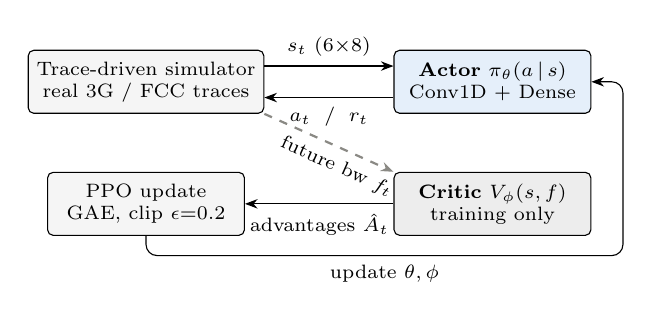
\begin{tikzpicture}[font=\scriptsize,
  box/.style={draw, rounded corners=2pt, align=center, inner sep=3pt, minimum height=8mm, minimum width=25mm},
  >={Stealth[length=1.6mm]}]
  \node[box, fill=gray!8] (sim) at (0,0) {Trace-driven simulator\\real 3G / FCC traces};
  \node[box, fill=ppo!12] (actor) at (4.4,0) {\textbf{Actor} $\pi_\theta(a\,|\,s)$\\Conv1D + Dense};
  \node[box, fill=priv!15] (critic) at (4.4,-1.55) {\textbf{Critic} $V_\phi(s,f)$\\training only};
  \node[box, fill=gray!8] (ppo) at (0,-1.55) {PPO update\\GAE, clip $\epsilon{=}0.2$};
  \draw[->] ([yshift=2mm]sim.east) -- node[above]{$s_t$ (6$\times$8)} ([yshift=2mm]actor.west);
  \draw[->] ([yshift=-2mm]actor.west) -- node[below]{$a_t$ \;/\; $r_t$} ([yshift=-2mm]sim.east);
  \draw[->, dashed, priv, thick] (sim.south east) -- node[pos=0.62, sloped, below, text=black]{future bw $f_t$} (critic.north west);
  \draw[->] (critic.west) -- node[below]{advantages $\hat A_t$} (ppo.east);
  \draw[->, rounded corners] (ppo.south) -- ++(0,-2.5mm) -| node[pos=0.25, below]{update $\theta,\phi$}
        ([xshift=4mm]actor.east) -- (actor.east);
\end{tikzpicture}
\caption{Training loop. The actor sees only what a real player sees. The critic additionally receives
the true future bandwidth $f_t$ from the simulator. It is discarded after training.}
\label{fig:arch}
\end{figure}

\textbf{Networks} (Pensieve-style). The scalar features feed Dense(128) layers. The three history rows and
the chunk-size row feed Conv1D(128, kernel 4) branches, which detect temporal patterns such as drops and
trends with shared weights. Everything is concatenated, passed through Dense(128), and then either a
softmax over 6 actions (actor, 266\,k parameters) or a scalar value (critic, 348\,k).

\textbf{Asymmetric critic.} Two states with an identical past can have very different futures, for
example a train about to \emph{enter} versus \emph{leave} a tunnel. A critic that sees only the past must
average them, which yields noisy advantages. Because the critic is needed only during training, we give it
\emph{privileged} information: the true mean bandwidth of the next $8\times4$\,s, read from the trace
(Fig.~\ref{fig:arch}). It still receives the actor's observation, which keeps the policy gradient unbiased
under partial observability [Baisero \& Amato 2022]. The deployed actor never sees the future.

\textbf{PPO.} Each rollout consists of 16 parallel simulators streaming one video each (768 transitions).
Advantages use GAE ($\gamma{=}0.99$, $\lambda{=}0.95$) with $V_\phi(s,f)$ and are normalised. The actor
maximises the clipped surrogate
$\mathbb{E}\big[\min(\rho_t\hat A_t,\operatorname{clip}(\rho_t,0.8,1.2)\hat A_t)\big]+\beta H(\pi_\theta)$
with $\rho_t=\pi_\theta/\pi_{\theta_\text{old}}$; the critic minimises $(G_t-V_\phi)^2$.
\begin{itemize}
  \item 4 epochs $\times$ 4 minibatches per rollout, stopped early if the approximate KL exceeds 0.03;
  \item entropy weight $\beta$: 0.1$\to$0.01;
  \item Adam (actor $10^{-4}$, critic $10^{-3}$), gradient clip 5;
  \item 10\,000 rollouts, about 1\,h on a laptop CPU;
  \item the best checkpoint is chosen on 12 held-out \emph{training} traces $\times$ 4 start points, never
    on test data.
\end{itemize}

\textbf{Why PPO.}
\begin{itemize}
  \item Tabular Q-learning cannot handle the continuous 25-dimensional state.
  \item DQN's max-operator overestimates under heavy-tailed stall penalties.
  \item A2C may take only one gradient step per rollout; PPO's clipping makes it safe to reuse each rollout
    4 times.
\end{itemize}
We first reproduced Pensieve's symmetric A2C (v1, v2). It serves as the control for the critic and
algorithm change.

\section{Baselines and Upper Bound}
\begin{itemize}
  \item \textbf{RB}: the highest bitrate below the harmonic mean of the last 5 throughputs.
  \item \textbf{BB} (BBA-0): buffer$\to$bitrate map with a 5\,s reservoir and a 10\,s cushion.
  \item \textbf{BOLA}: a Lyapunov utility rule.
  \item \textbf{FastMPC/RobustMPC}: exhaustive search over all $6^5$ plans for the next 5 chunks with
    predicted bandwidth; RobustMPC discounts by the maximum recent prediction error.
  \item \textbf{Offline optimal}: dynamic programming over (last bitrate, buffer in 0.5\,s bins) with
    \emph{full knowledge} of the trace. It is an unreachable upper bound and converges to within 0.01 QoE
    across bin sizes.
\end{itemize}



\section{Results}
Table~\ref{tab:results} compares all methods.

\textbf{PPO beats every baseline on every test set.} Against RobustMPC, the strongest heuristic:
\begin{itemize}
  \item QoE is \textbf{+7\,\%} on HSDPA, \textbf{+12\,\%} on FCC and \textbf{+89\,\%} on the stress tests;
  \item stall time is $2.6\times$ lower and quality switches are $2.1\times$ fewer.
\end{itemize}
PPO closes 27\,\% of the gap between RobustMPC and the offline optimum. In the metro tunnel, RobustMPC's
throughput predictor extrapolates the good past right into a 0\,Mbps outage ($-1.79$). PPO, having
experienced such drops in real traces, keeps a buffer reserve (1.37).

Fig.~\ref{fig:ts} shows how PPO wins. Like the optimum, it builds a large buffer while bandwidth is good;
the heuristics keep a thin buffer and stall repeatedly when the bandwidth collapses. It also shows a
remaining weakness: PPO requests one high-bitrate chunk just as the link degrades.

\textbf{RL ablation} (Fig.~\ref{fig:train}).
\begin{itemize}
  \item A2C v1's entropy bonus ($\beta{=}1.0$) dominated the normalised advantages. Its policy stayed
    uniform ($H{=}\ln6$) for half of training, and it ended only 3\,\% above RobustMPC.
  \item Lowering $\beta$ (v2) sped up learning, but the noisy 12-video validation selected a weaker
    checkpoint.
  \item PPO with the privileged critic, sample reuse and a 48-video validation set becomes decisive
    steadily and gives the best policy on all test sets.
\end{itemize}



\begin{figure}[t]
\centering
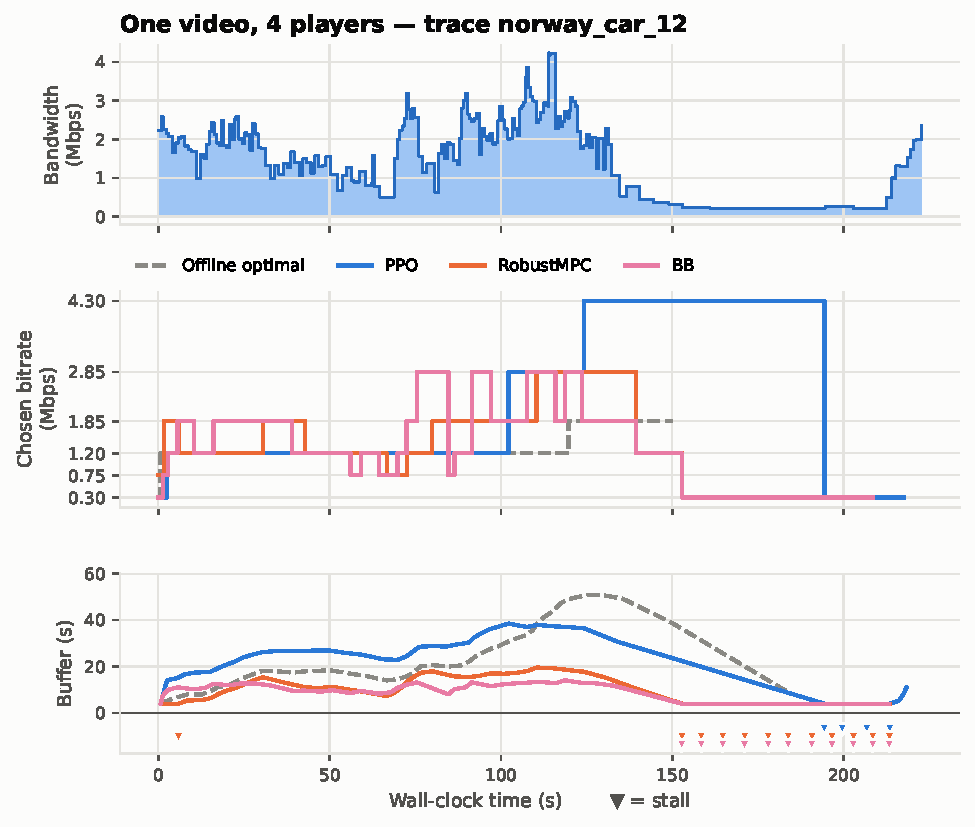
\includegraphics[width=0.72\columnwidth]{g5_timeseries_hsdpa_test.pdf}
\caption{One HSDPA test video. Top: bandwidth. Middle: chosen bitrate. Bottom: buffer (\(\blacktriangledown\) = stall).}
\label{fig:ts}
\end{figure}

\begin{figure}[t]
\centering
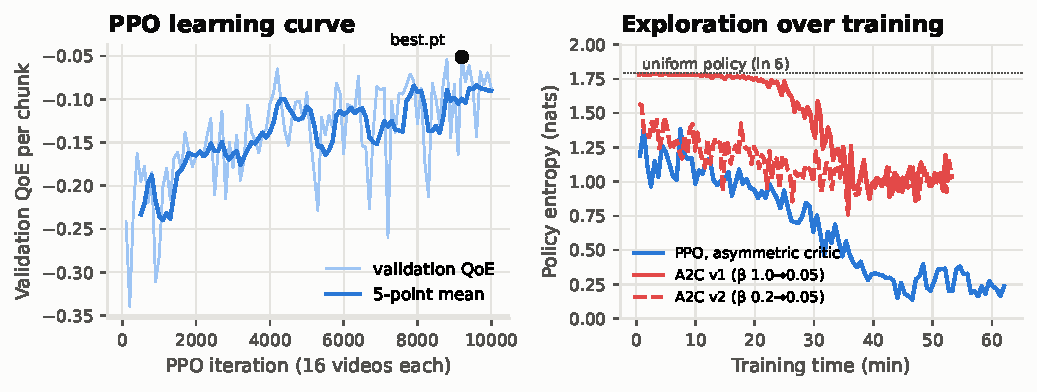
\includegraphics[width=\columnwidth]{g1_training.pdf}
\caption{Left: PPO validation QoE (negative because the validation traces contain unavoidable FCC
outages). Right: policy entropy vs.\ training time. A2C v1 stays near-uniform for about 30\,min.}
\label{fig:train}
\end{figure}

\textbf{Limitations.}
\begin{itemize}
  \item Traces are open-loop: there is no TCP or congestion feedback from the player's own traffic.
  \item Only one test video is used.
  \item QoE$_\text{lin}$ is a simplified model of perception.
\end{itemize}
The repository contains the full pipeline: simulator, baselines, training, the trained agent, 38 tests
and a web demo where you can draw a network and watch PPO stream next to the baselines.

\vspace{-0.4em}
\begin{thebibliography}{9}\footnotesize
\setlength{\itemsep}{0pt}
\bibitem{pensieve} H.~Mao, R.~Netravali, M.~Alizadeh. Neural adaptive video streaming with Pensieve. SIGCOMM 2017.
\bibitem{mpc} X.~Yin, A.~Jindal, V.~Sekar, B.~Sinopoli. A control-theoretic approach for dynamic adaptive video streaming over HTTP. SIGCOMM 2015.
\bibitem{bba} T.-Y.~Huang et al. A buffer-based approach to rate adaptation. SIGCOMM 2014.
\bibitem{bola} K.~Spiteri, R.~Urgaonkar, R.~Sitaraman. BOLA: near-optimal bitrate adaptation for online videos. INFOCOM 2016.
\bibitem{ppo} J.~Schulman et al. Proximal policy optimization algorithms. arXiv:1707.06347, 2017.
\bibitem{asym} L.~Pinto et al. Asymmetric actor critic for image-based robot learning. RSS 2018.
\bibitem{unbiased} A.~Baisero, C.~Amato. Unbiased asymmetric reinforcement learning under partial observability. AAMAS 2022.
\bibitem{hsdpa} H.~Riiser et al. Commute path bandwidth traces from 3G networks. MMSys 2013.
\end{thebibliography}

\end{document}
